%! Author = Wiktor Rostkowski, Mateusz Budzisz
%! Date = 29/04/2024

\chapter{Projekt}
\label{ch:projekt}

\section{Wzorce projektowe}\label{sec:wzorce-projektowe}
W projekcie wykorzystano następujące wzorce projektowe:
\begin{itemize}

    \item \textbf{MVVM (Model-View-ViewModel)}: Wzorzec architektoniczny, który oddziela logikę biznesową (Model) od interfejsu użytkownika (View) za pomocą warstwy pośredniej (ViewModel), która zarządza stanem i~logiką prezentacji.

    \item \textbf{MVC (Model-View-Controller)}: Wzorzec projektowy, który dzieli aplikację na trzy główne komponenty: Model (logika danych), View (interfejs użytkownika) i~Controller (logika aplikacji).
    Pozwala to na lepsze zarządzanie kodem i~jego modularność.

    \item \textbf{REST API (Representational State Transfer Application Programming Interface)}: Styl architektoniczny dla systemów rozproszonych, oparty na protokole HTTP, który umożliwia komunikację między klientem a serwerem za pomocą standardowych metod (GET, POST, PUT, DELETE).

    \item \textbf{Repository}: Wzorzec projektowy, który zapewnia warstwę abstrakcji nad dostępem do danych.
    Umożliwia oddzielenie logiki biznesowej od warstwy dostępu do danych, co ułatwia zarządzanie danymi i~testowanie aplikacji.

    \item \textbf{Dependency Injection}: Technika polegająca na wstrzykiwaniu zależności do komponentów, zamiast tworzenia ich wewnątrz komponentów.
    Umożliwia to luźne powiązanie między komponentami i~ułatwia testowanie oraz zarządzanie zależnościami.

    \item \textbf{Redux}: Wzorzec do zarządzania stanem aplikacji, szczególnie popularny w aplikacjach React.
    Opiera się na centralnym magazynie (store), który przechowuje cały stan aplikacji, oraz na akcjach i~reduktorach, które modyfikują ten stan w kontrolowany sposób.

    \item \textbf{Observer}: Wzorzec projektowy, w którym obiekt (obserwowany) powiadamia inne obiekty (obserwatorów) o zmianach swojego stanu.
    Umożliwia to reaktywne programowanie i~luźne powiązanie między obiektami.

    \item \textbf{Reverse Proxy}: Serwer pośredniczący, który przyjmuje żądania od klientów i~przekazuje je do odpowiednich serwerów docelowych.
    Używany do zwiększenia wydajności, równoważenia obciążenia i~poprawy bezpieczeństwa.

    \item \textbf{Bearer Token}: Metoda autoryzacji, w której token dostępu jest przesyłany w nagłówku HTTP\@.
    Umożliwia to bezpieczne uwierzytelnianie użytkowników i~autoryzację dostępu do zasobów.

    \item \textbf{Service}: Pojęcie szerokie, odnoszące się do jednostki funkcjonalnej w aplikacji, która realizuje określoną usługę.

\end{itemize}

\section{Komponenty}\label{sec:komponenty}
W skład systemu wchodzą:
\begin{itemize}
    \item Progresywna aplikacja webowa (PWA)
    \item Backend zgodny ze standardem REST API
    \item Baza danych PostgreSQL
\end{itemize}

\section{Architektura}\label{sec:architektura}
System został zbudowany w architekturze monolitycznej, co oznacza, że wszystkie jego elementy i~funkcjonalności są zintegrowane w jednym serwisie, zamiast być podzielone na niezależne moduły lub mikroserwisy.
System został wdrożony w chmurze obliczeniowej Oracle Ampere.
Aby uniknąć problemów z CORS (Cross-Origin Resource Sharing), wszystkie połączenia przychodzące z różnych źródeł są przekierowywane przez serwer Nginx.
Nginx działa jako reverse proxy, który odpowiednio kieruje ruch do właściwych komponentów systemu znajdujących się na serwerze.
Dzięki temu z perspektywy użytkownika wszystkie usługi systemu są dostępne pod tym samym adresem URL\@.
Dodatkowo, użycie Nginx umożliwia łatwe wygenerowanie certyfikatu SSL za pomocą Let's Encrypt, co zapewnia bezpieczne połączenia HTTPS i~chroni dane użytkowników przed potencjalnymi zagrożeniami.

\begin{figure}[H]
    \centering
    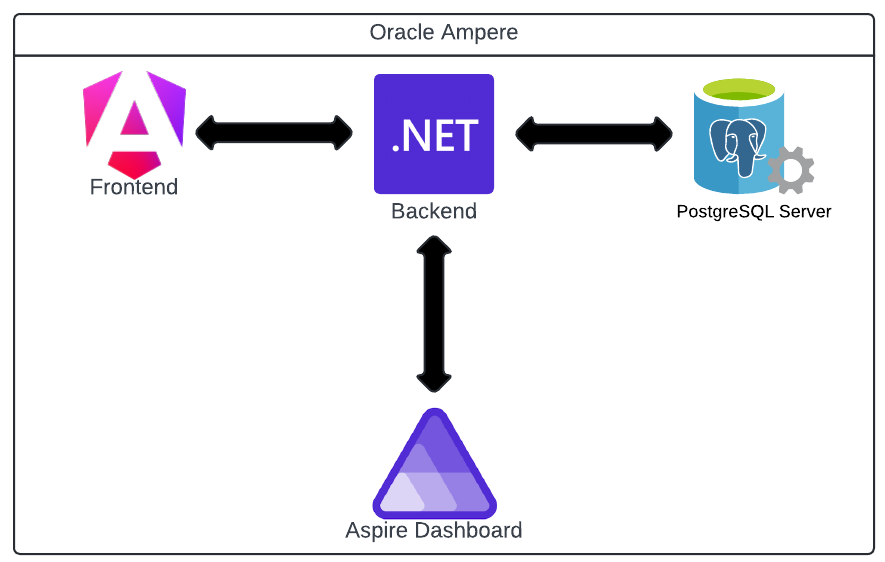
\includegraphics[width=1\textwidth]{attachments/arch-diag}
    \caption{Diagram systemu w środowisku docelowym}
    \label{fig:figure}
\end{figure}

